\documentclass[a4paper, 12pt]{article}
\usepackage[a4paper,top=1.5cm, bottom=1.5cm, left=1cm, right=1cm]{geometry}

% Работа с русским языком
\usepackage[utf8]{inputenc}
\usepackage{mathtext}                % русские буквы в формулах
\usepackage[english, russian]{babel} % локализация и переносы

\usepackage{graphicx}   % Вставка изображений
\usepackage{float}      % "Плавающие" изображения3
\usepackage{wrapfig}    % Обтекание фигур (таблиц, картинок и прочего)
\usepackage{subfig}
\graphicspath{ {./images/} }

\usepackage{tabularx}
\usepackage{multirow}
\usepackage{amsmath}
\usepackage{amsfonts}
\usepackage{indentfirst}
\usepackage{longtable}
\graphicspath{{pictures/}}
\usepackage{natbib}
\usepackage{bm}

%%% Колонтитулы
\usepackage{titleps}
\newpagestyle{main}{
	\setheadrule{0.4pt}
	\sethead{Закон Кюри-Вейса}{}{}
	\setfootrule{0.4pt}                       
	\setfoot{ФРКТ МФТИ, 2023}{}{\thepage} 
}
\pagestyle{main}  

\begin{document}
    \begin{titlepage}
	\begin{center}
            {\large МОСКОВСКИЙ ФИЗИКО-ТЕХНИЧЕСКИЙ ИНСТИТУТ (НАЦИОНАЛЬНЫЙ ИССЛЕДОВАТЕЛЬСКИЙ УНИВЕРСИТЕТ)}
	\end{center}
 
	\begin{center}
		{\large Физтех-школа радиотехники и компьютерных технологий}
	\end{center}
	
	\vspace{8cm}
	{\LARGE
		\begin{center}
                {\bf Отчёт о выполнении лабораторной работы 3.4.2}\\
                Закон Кюри-Вейса
		\end{center}
	}
	\vspace{5cm}
	\begin{flushright}
		{\Large Автор:\\ Тихонов Дмитрий Романович, \\
			\vspace{0.2cm}
			студент группы Б01-206}
	\end{flushright}
	\vspace{5cm}
	\begin{center}
		\Large Долгопрудный, 2023
	\end{center}
    \end{titlepage}


    \section{Введение}

    \noindent \textbf{Цель работы:} изучение температурной зависимости магнитной восприимчивости ферромагнетика выше точки Кюри. \\

    \noindent \textbf{В работе используются:} катушка самоиндукции с образцом из гадолиния, термостат, частотомер, цифровой вольтметр, $LC$-автогенератор, термопара медь-константан.
    
    \section{Теоретические сведения}
    
    Вещества с отличными от нуля атомными магнитными моментами обладают парамагнитными свойствами. Внешнее магнитное поле ориентирует магнитные моменты, которые в отсутствие поля располагались в пространстве хаотичным образом. При повышении температуры $Т$ возрастает дезориентирующее действие теплового движения частиц, и магнитная восприимчивость парамагнетиков убывает по \textit{закону Кюри} -- обратно пропорционально температуре:

    \begin{equation}
        \chi \propto \frac{1}{T}.
    \end{equation}
    
    Некоторые парамагнетики при понижении температуры испытывают фазовый переход в ферромагнитное состояние. При малых температурах тепловое движение всё меньше препятствует магнитным моментам атомов ориентироваться в одном направлении при сколь угодно слабом внешнем поле. Благодаря обменному взаимодействию, имеющему электростатическую природу, в ферромагнетиках самопроизвольное упорядочение магнитных моментов возможно при довольно высоких температурах. Температуру фазового перехода парамагнетик-ферромагнетик называют \textit{температурой Кюри} $\Theta_K$. Температурная зависимость магнитной восприимчивости у ферромагнетиков выше точки Кюри с удовлетворительной точностью описывается \textit{законом Кюри-Вейсса}:

    \begin{equation}
        \chi \propto \frac{1}{T - \Theta_p},
        \label{eq:Curie_Weiss}
    \end{equation}
    
    где $\Theta_p$ -- параметр с размерностью температуры, называемый иногда \textit{парамагнитной точкой Кюри}. Величина $\Theta_p$ близка к $\Theta_K$, но не совпадает с ней.
    
    Непосредственно вблизи $\Theta_K$ закон Кюри-Вейсса (\ref{eq:Curie_Weiss}) нарушается. На практике наблюдается зависимость, изображённая на рис. \ref{gd:Curie_Weiss}.

    \begin{figure}[H]
        \centering
        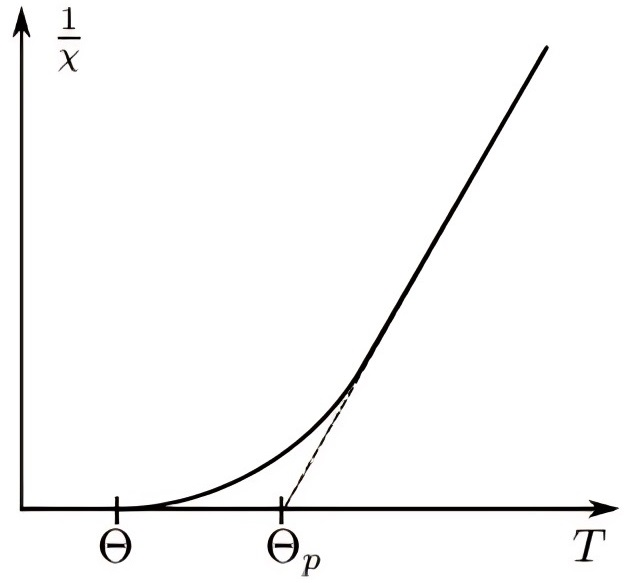
\includegraphics[scale = 0.7]{images/Curie_Weiss.png}
        \caption{Теоретическая зависимость обратной магнитной восприимчивости от температуры}
        \label{gd:Curie_Weiss}
    \end{figure}
    
    \section{Методика измерений и экспериментальная установка}
    
    Схема установки для проверки закона Кюри-Вейсса показана на рис. \ref{installation}. Исследуемый ферромагнитный образец (гадолиний) расположен внутри пустотелой катушки самоиндукции, которая служит индуктивностью колебательного конутра, входящего в состав $LC$-автогенератора.

    \begin{figure}[H]
        \centering
        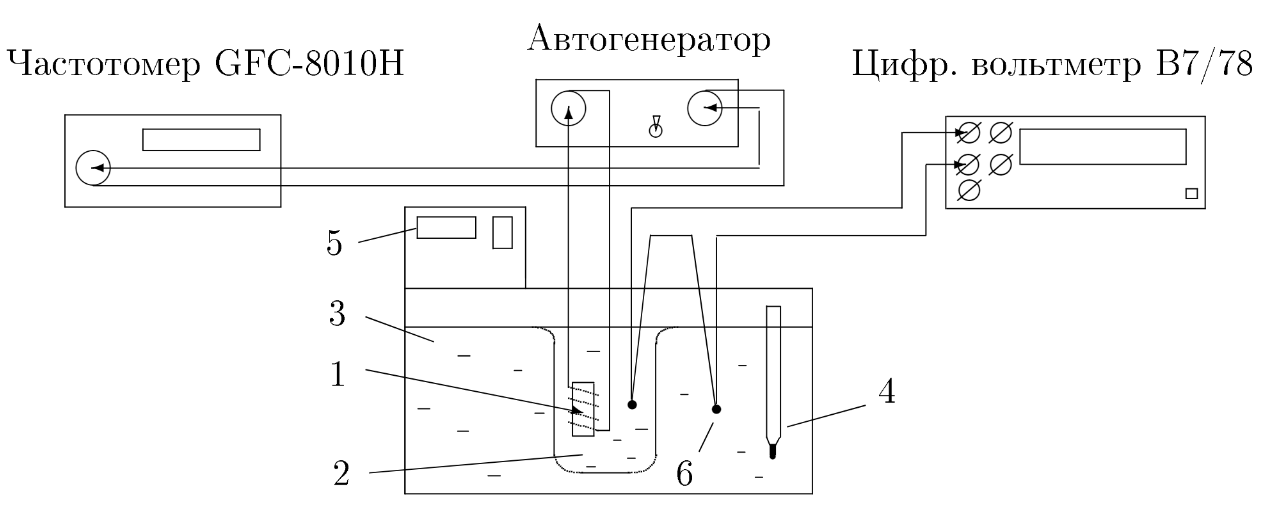
\includegraphics[width = 14 cm]{images/installation.png}
        \caption{Схема экспериментальной установки}
        \label{installation}
    \end{figure}
	
    Магнитная воосприимчивость образца $\chi$ определяется по изменению самоиндукции катушки. Обозначив через $L$ самоиндукцию катушки с образцом, а $L_0$ -- её самоиндукцию в отсутствие образца, получим
    
    \begin{equation}
        (L - L_0) \propto \mu - 1 = \chi.
    \end{equation}
    
    При изменении самоиндукции образца меняется период колебаний автогенератора:
    
    \begin{equation}
        \tau = 2\pi \sqrt{LC},
    \end{equation}
    
    где $C$ -- ёмкость контура автогенератора. Период колебаний в отсутствие образца определяется самоиндукцией пустой катушки:
    
    \begin{equation}
        \tau_0 = 2\pi \sqrt{L_0C}.
    \end{equation}

    Остюда находим

    \begin{equation}
        L - L_0 \propto \tau^2 - \tau_0^2 \Rightarrow \chi \propto \tau^2 - \tau_0^2.
        \label{eq:exp}
    \end{equation}
    
    Из формул (\ref{eq:Curie_Weiss}) и (\ref{eq:exp}) следует, что закон Кюри-Вейсса \textit{справедлив}, если выполнено соотношение
    
    \begin{equation}
        \frac{1}{\tau^2 - \tau_0^2} \propto T - \Theta_p.
    \end{equation}

    Температура исследуемого образца всегда несколько отличается от температуры воды в термостате. После того как вода достигла заданной температуры, идёт медленный процесс выравнивания температур образца и воды. Разность их температур контролируется с помощью медно-константановой термопары $6$, один из спаев которой находится в тепловом контакте с образцом, а другой погружён в воду. Измерение периода колебаний автогенератора проводились в тот момент, когда указанная разность температур становилась меньше $0,5 \: ^\circ$C, т.к. \textit{более точному измерению температур мешают паразитные ЭДС}, возникающие в цепи термопары.
	
    \section{Результаты измерений и обработка данных}

    \begin{enumerate}
        \item Подготовим приборы к работе. Оценим допустимую ЭДС термопары: $\Delta U = \frac{\Delta T}{k} = 0,0208$ мВ, где $k = 24 \: ^\circ$C/мВ и $\Delta T = 0.5 \: ^{\circ}$С.
        
        \item Исследуем зависимость периода колебания генератора от температуры образца, отмечая период колебаний $\tau$ по частотомеру, а температуру $T$ -- по показаниям дисплея и цифровому вольтметру. Занесём в таблицу \ref{table:results} измеренные и рассчитанные значения.

        \begin{table}[H]
            \centering
            \begin{tabular}{|c|c|c|c|c|c|c|}
            \hline
            $T'$, $^\circ$C  & $\tau$, мкс & $\tau_0$, мкс & $\Delta U$, мВ & $\Delta T$, $^\circ$C & $1/(\tau^2 - \tau_0^2), \text{мкс}^{-2} $ & $T$, $^\circ$C \\ \hline
            14,12 & 10,789 & \multirow{14}{*}{9,045} & -0,0118 & -0,28 & 0,029 & 13,84 \\ \cline{1-2} \cline{4-7} 
            16,09 & 10,692 &  & -0,0105 & -0,25 & 0,031 & 15,84 \\ \cline{1-2} \cline{4-7} 
            18,09 & 10,527 &  & -0,0109 & -0,26 & 0,034 & 17,83 \\ \cline{1-2} \cline{4-7} 
            20,10 & 10,225 &  & -0,0086 & -0,21 & 0,044 & 19,89 \\ \cline{1-2} \cline{4-7} 
            22,11 & 9,926 &  & -0,0153 & -0,37 & 0,060 & 21,74 \\ \cline{1-2} \cline{4-7} 
            24,10 & 9,617 &  & -0,0195 & -0,47 & 0,094 & 23,63 \\ \cline{1-2} \cline{4-7} 
            26,00 & 9,455 &  & -0,0159 & -0,38 & 0,132 & 25,62 \\ \cline{1-2} \cline{4-7} 
            28,16 & 9,366 &  & -0,0155 & -0,37 & 0,169 & 27,79 \\ \cline{1-2} \cline{4-7} 
            30,02 & 9,322 &  & -0,0175 & -0,42 & 0,197 & 29,60 \\ \cline{1-2} \cline{4-7} 
            32,03 & 9,286 &  & -0,0161 & -0,39 & 0,226 & 31,64 \\ \cline{1-2} \cline{4-7} 
            34,01 & 9,261 &  & -0,0184 & -0,44 & 0,253 & 33,57 \\ \cline{1-2} \cline{4-7} 
            36,12 & 9,241 &  & -0,0181 & -0,43 & 0,279 & 35,69 \\ \cline{1-2} \cline{4-7} 
            38,05 & 9,226 &  & -0,0187 & -0,45 & 0,302 & 37,60 \\ \cline{1-2} \cline{4-7} 
            40,07 & 9,212 &  & -0,0065 & -0,16 & 0,328 & 39,91 \\ \hline
            \end{tabular}
            \caption{Результаты исследования зависимости периода колебания генератора от температуры образца}
            \label{table:results}
        \end{table}
    
        \item Построим график зависимости $\frac{1}{(\tau^2-\tau_0^2)} = f(T)$. Прямую ферромагнитного участка экстраполируем к оси абсцисс, полученное значение -- экспериментальное значение точки Кюри для исследуемого образца. 
    
        \begin{figure}[H]
            \centering
            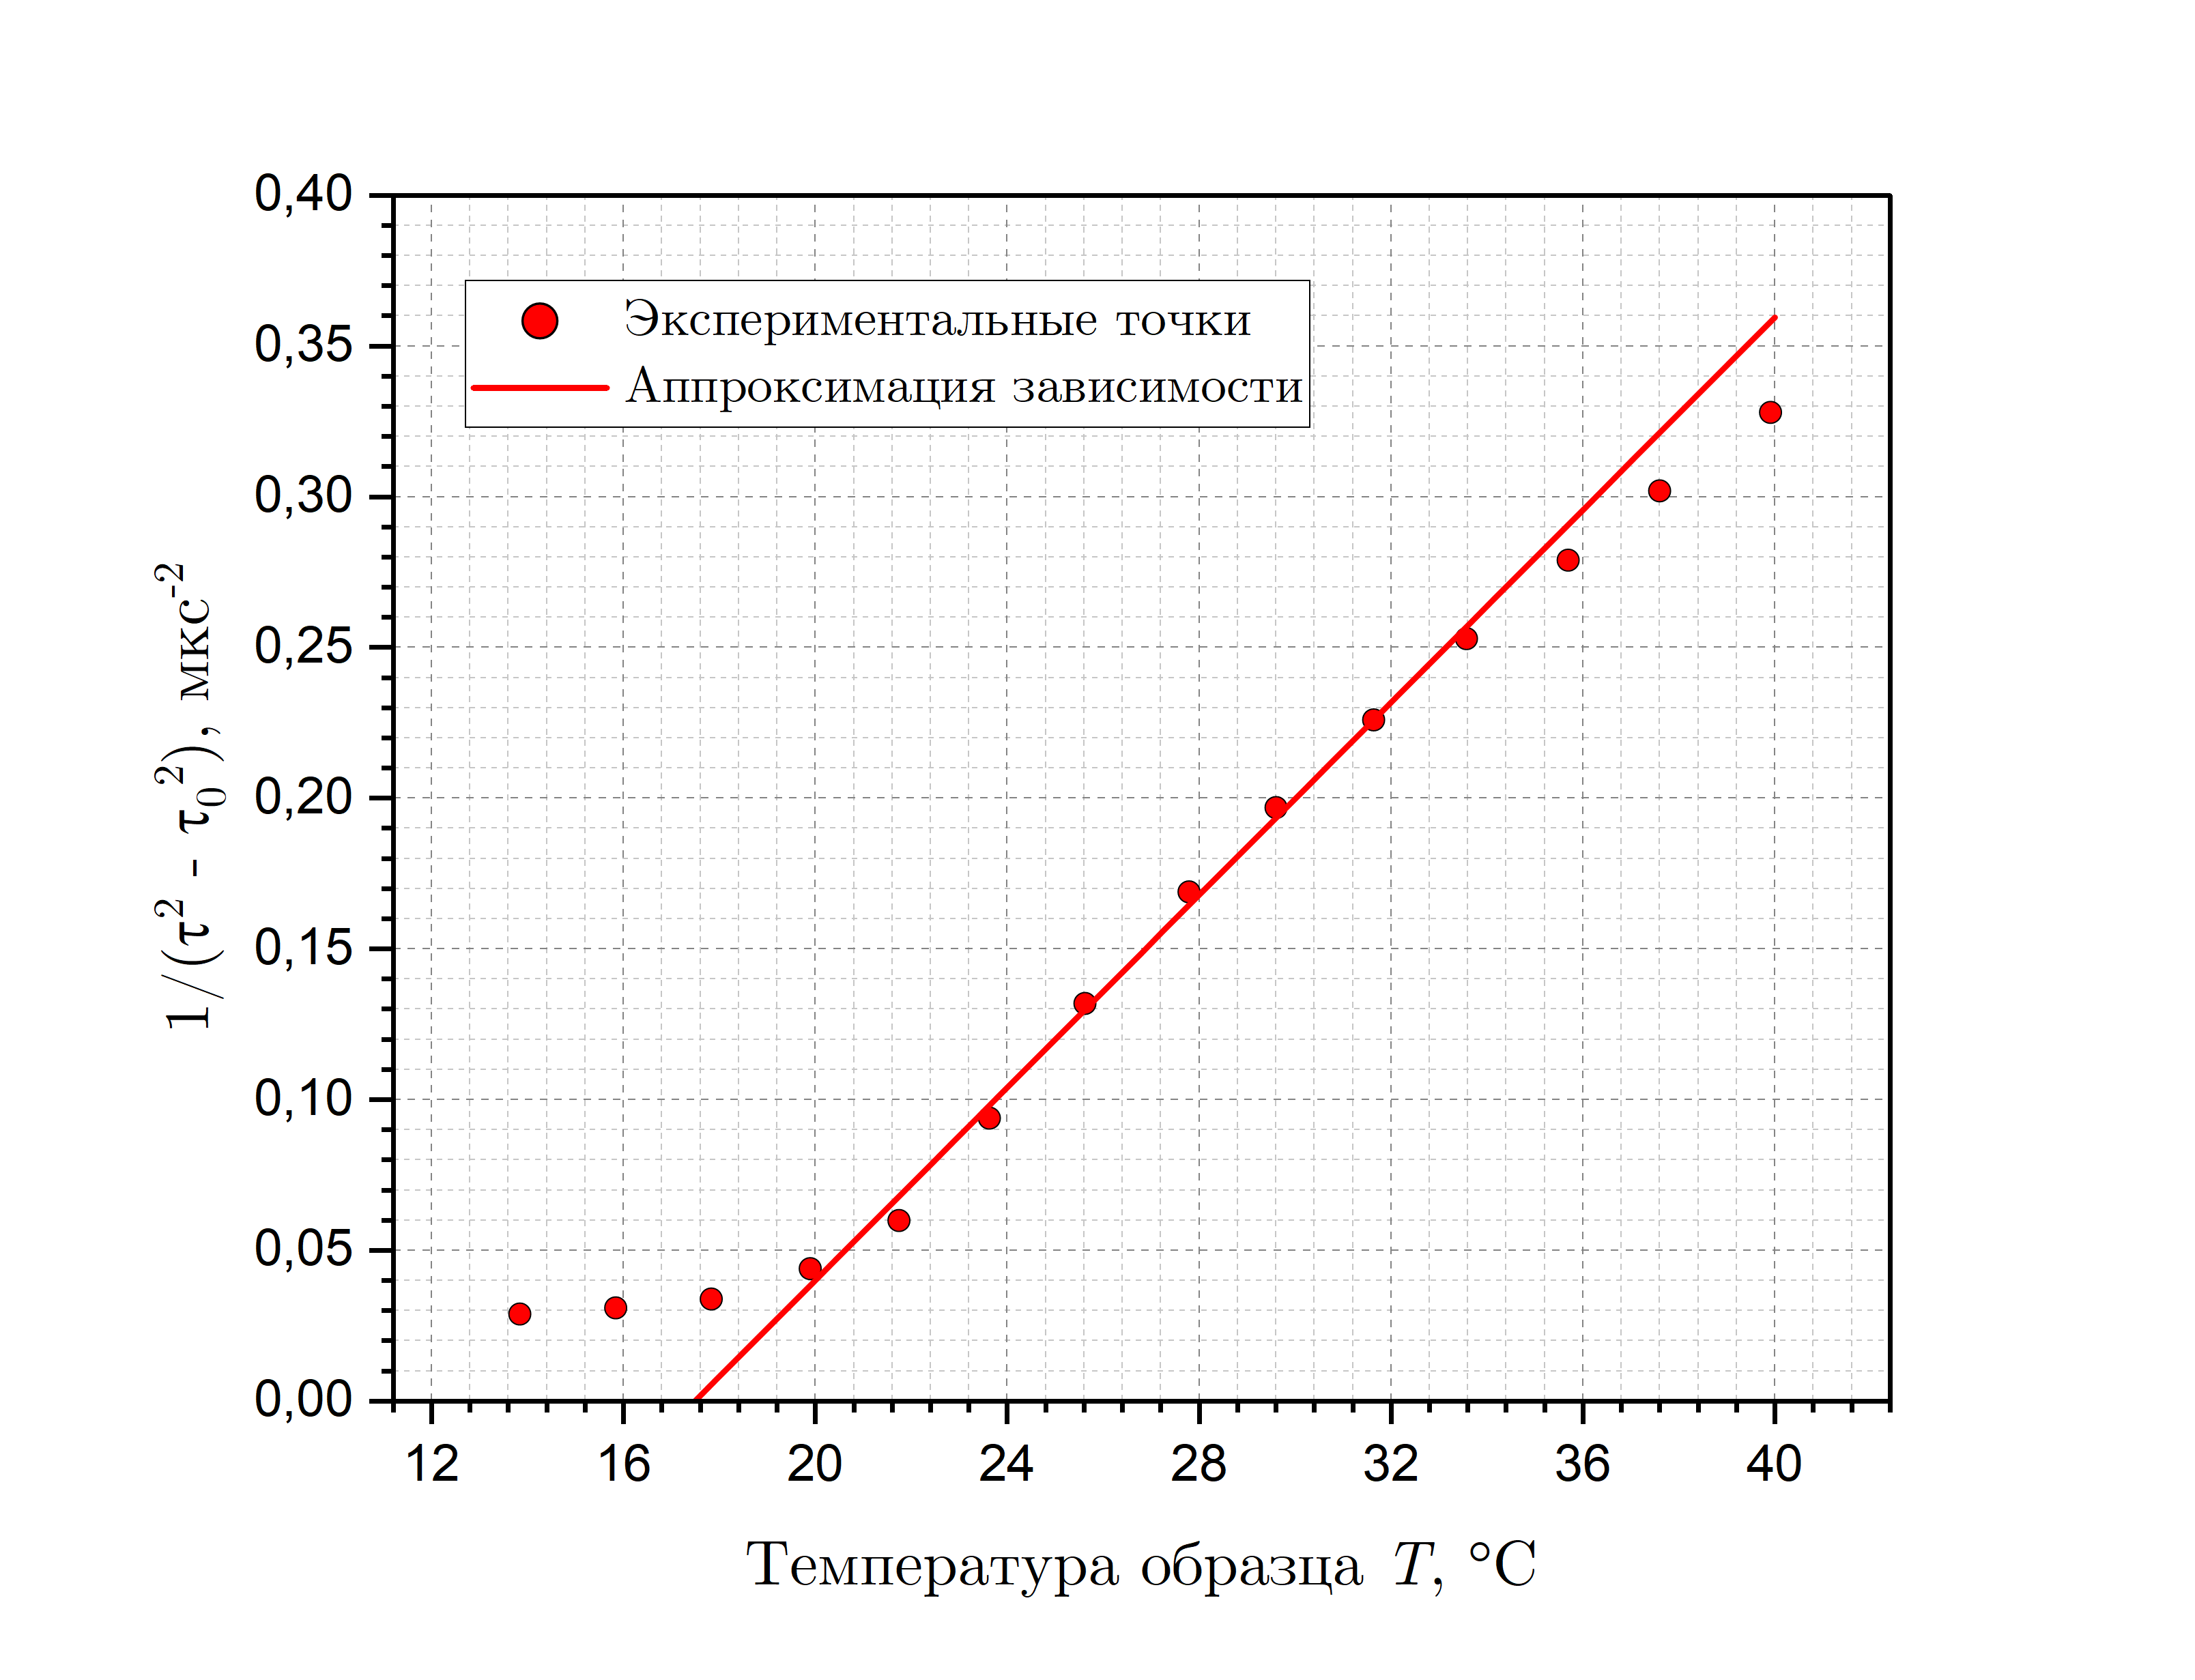
\includegraphics[scale = 0.45]{images/graph_Curie_Weiss.png}
            \caption{Зависимость $\frac{1}{(\tau^2-\tau_0^2)} = f(T)$}
            \label{graph}
        \end{figure}
    
        \item Аппроксимируя полученные данные при помощи программы \textit{OriginPro 2023b}, получим \textit{значение парамагнитной точки Кюри для гадолиния} $\Theta_p = \left( 17,5 \pm 0,8 \right) \: ^{\circ}$C и \textit{значение температуры Кюри для гадолиния} $\Theta_p \approx 20 \: ^{\circ}$C.
    \end{enumerate}

    
    \section{Заключение}

    \begin{enumerate}
        \item В ходе работы был экспериментально \textit{подтвержден закон Кюри-Вейсса} для металла гадолиния. 
        
        \item Была найдена \textit{температура Кюри}: $\Theta_K \approx 20 \: ^\circ$C. Полученное значение отличается от табличного $\Theta_p^\text{табл} = 20,2 \: ^\circ$C на $1 \%$.

        \item Была найдена \textit{парамагнитная температура Кюри}: $\Theta_p = \left( 17,5 \pm 0,8 \right) \: ^{\circ}$C. Заметим, что \textit{парамагнитная температура Кюри меньше температуры Кюри} ($\Theta_p < \Theta_K$).

        \item Основной вклад в погрешность внесла неточность данных, полученных при температурах, близких к температуре Кюри.

        \item Анализ погрешностей показал, что измерения были проведены с достаточной точностью.
    \end{enumerate}

\end{document}